% Copyright 2026 Sreeram Anil
% SPDX-License-Identifier: CC-BY-4.0
% =============================================================================
%  Decentralised pack filtering (baseline) — pack-level family
% =============================================================================
\chapter{Decentralised Pack Filtering (Decentralized-EKF)}
\label{ch:decentralizedekf}

\section*{At a glance}
\begin{tabular}{@{}l>{\raggedright\arraybackslash}p{0.76\textwidth}@{}}
Family & pack-level (baseline: no information exchange) \\
Header & \texttt{include/estkit/pack/pack\_estimator.hpp} (\texttt{DecentralizedPack<Filter>}) \\
Registered name & \texttt{Decentralized-EKF} \\
Structure & $N_c$ independent 4-state EKFs, one per cell \\
Cost per step & \SI{3860}{\nano\second} for $N_c=12$ cells (\SI{322}{\nano\second} per cell) \\
Memory & \SI{52032}{\byte} $= N_c\times\SI{4336}{\byte}$ \\
Bus load & 0 \\
Primary references & \cite{plett2004ekf3,plett2016bms2,plett2015bms1} \\
\end{tabular}

\section{Motivation and aerospace/BMS relevance}
This chapter describes the reference point of the pack-level family: apply the cell-level
estimator of Chapter~\ref{ch:ekf} independently to every cell of the module, and report its
output as that cell's SOC. It is the architecture a BMS gets ``for free'' once a cell-level filter
exists --- no pack model, no inter-cell assumptions, no communication --- and it is the only
member of this family that makes no structural assumption about the pack at all. Every other
chapter of the family must justify itself against it, both in accuracy and in cost.

It is also a genuinely defensible design. Each cell-monitor slave runs its own filter on its own
voltage channel; a failed channel affects exactly one cell's estimate; there is no master, no bus
traffic and no shared state to corrupt. For a small pack, or for a pack whose cells are wired in
parallel (where the shared-current assumption of Chapters~\ref{ch:bardelta}--\ref{ch:consensus}
fails), it is the correct choice. Its weaknesses are quantitative rather than structural: it costs
$N_c$ times a cell filter, and it extracts the state of charge of each cell from one noisy voltage
channel when $N_c$ channels observe almost the same quantity.

\section{Problem statement and assumptions}
A module of $N_c$ cells in series, common current $i_k$, per-cell voltages $v_{j,k}$ and
temperatures $T_{j,k}$ (notation of Chapter~\ref{ch:bardelta}). The estimator carries $N_c$
independent states
\begin{equation}
\vx_{j,k} = [\soc_{j,k},\,v_{1,j,k},\,v_{2,j,k},\,h_{j,k}]^\T\in\real^{4},\qquad j=1,\dots,N_c,
\label{eq:dek-state}
\end{equation}
each propagated by the ESC model of Chapter~\ref{ch:ecm} with the \emph{nominal} parameter set ---
the estimator is not told the per-cell spread --- and each corrected by its own voltage channel.

\begin{assumption}[No cross-cell information]\label{as:dek-nocross}
The $N_c$ estimation problems are treated as independent. This is correct for the measurement
noises (Assumption~\ref{as:if-indep}) but wrong for the states: all cells share $i_k$, so their
errors are strongly correlated and the decentralised filter cannot exploit that.
\end{assumption}

\section{Derivation}
There is nothing to derive beyond Chapter~\ref{ch:ekf}: cell $j$ runs
\begin{align}
\vx^-_{j,k} &= f(\vx^+_{j,k-1},\vu_{j,k-1}), &
\Pminus_{j,k} &= \mF_j\Pplus_{j,k-1}\mF_j^\T + \mQ_j, \label{eq:dek-tu}\\
\mK_{j,k} &= \Pminus_{j,k}\mH_j^\T\big(\mH_j\Pminus_{j,k}\mH_j^\T+R\big)\inv, &
\vx^+_{j,k} &= \vx^-_{j,k}+\mK_{j,k}\big(v_{j,k}-h(\vx^-_{j,k},\vu_{j,k})\big),
\label{eq:dek-mu}
\end{align}
with $\vu_{j,k}=[i_k,T_{j,k}]^\T$ and the Joseph-form covariance update, and reports
$\hat\soc_{j,k} = \vx^+_{j,k}[1]$. The pack-level quantities follow directly:
$\min_j\hat\soc_j$, $\max_j\hat\soc_j$, $N_c^{-1}\sum_j\hat\soc_j$.

The interesting statement is what this \emph{cannot} do. Write the SOC error of cell $j$ as
$\tilde\soc_j$. The current-sensor error $\delta i_k$ enters every cell identically, so the
coulomb-counting part of $\tilde\soc_j$ contains the common term
$-\eta\dt\,\delta i_k/(3600 Q)$ for all $j$; the voltage-sensor noise $e_{j,k}$ enters each cell
independently. A decentralised filter must reject both with the same gain. A common-state
estimator can average the $N_c$ independent $e_{j,k}$ down by $\sqrt{N_c}$ before applying a gain
--- which is exactly the factor that separates the two columns of the benchmark table below.
Conversely, no architecture can average the common $\delta i_k$ down, which is why
\texttt{current\_bias} is the scenario in which all pack-level methods are closest together.

\section{Algorithm}
\begin{algorithm}[H]
\caption{Decentralized-EKF --- one sampling period $k$}
\begin{algorithmic}[1]
\Require $\{\vx^+_{j,k-1},\Pplus_{j,k-1}\}_{j=1}^{N_c}$, $i_k$, $\{v_{j,k}\}$, $\{T_{j,k}\}$
\ForAll{cells $j = 1,\dots,N_c$ \textbf{in parallel, no communication}}
  \State $\vu_{j,k}\gets[i_k,T_{j,k}]^\T$
  \State time update \eqref{eq:dek-tu} with $\vu_{j,k-1}$
  \State measurement update \eqref{eq:dek-mu} with $v_{j,k}$; constrain $\soc\in[-0.05,1.05]$, $|h|\le1$
\EndFor
\Ensure $\hat\soc_{j,k}$, $j=1,\dots,N_c$
\end{algorithmic}
\end{algorithm}

\section{Application to the battery model}
\texttt{DecentralizedPack<Filter>} owns $N_c$ \texttt{CellEstimator<Filter>} objects and forwards
\texttt{step(i, v[j], T[j])} to each; the timing convention (predict with $\vu_{k-1}$, then update
with $\vy_k,\vu_k$) is the one of Chapter~\ref{ch:ekf}. Every cell filter uses the identical
nominal \texttt{CellParams}, the identical $\mQ$ (current-sensor noise mapped through $\partial
f/\partial i$ plus the diagonal floor) and $R=\sigma_v^2+(R_0\sigma_i)^2$. No option is tuned at
pack level: this is the cell-level EKF, twelve times.

\section{Implementation notes}
The container holds \texttt{std::unique\_ptr<CellEstimator<Filter>>} objects created once at
construction; the hot path (\texttt{step}) allocates nothing. Memory is
$N_c\,\texttt{sizeof(Ekf<EcmModel>)} = 12\times\SI{4336}{\byte} = \SI{52032}{\byte}$, of which
$12\times\SI{3872}{\byte}$ is twelve private copies of the 241-point OCV table --- in a real BMS
one shared read-only table, leaving \SI{464}{\byte} of RAM per cell. Timing is
\SI{322}{\nano\second} per cell per sample, i.e.\ exactly the cell-level EKF of
Chapter~\ref{ch:ekf}; on $N_c$ processors the wall-clock cost is that figure, on one processor it
is $N_c$ times larger.

\emph{Limitations.} It scales linearly in $N_c$ in both time and memory, and it is the least
accurate architecture of this family on every scenario. It has no notion of the pack, so it
cannot report ``how far apart are my cells'' any more accurately than the difference of two
independently noisy estimates.

\section{Benchmark results}
% Copyright 2026 Sreeram Anil
% SPDX-License-Identifier: CC-BY-4.0
\begin{table}[H]\centering\footnotesize\setlength{\tabcolsep}{4pt}\caption{Decentralized-EKF: pack-level benchmark (12-cell module, eVTOL mission, mean over seeds; all errors in \% SOC). RMSE$_\mathrm{cells}$: per-cell RMSE over all cells; RMSE$_{\min/\mathrm{mean}/\max}$: error of the weakest / mean / strongest-cell SOC; 52032 bytes of state, 0 numbers exchanged per step.}\label{tab:pack_DecentralizedEKF}
\begin{tabular}{lrrrrrrcr}\toprule scenario & RMSE$_\mathrm{cells}$ & RMSE$_{\min}$ & RMSE$_\mathrm{mean}$ & RMSE$_{\max}$ & max cell err. & RMSE$_\mathrm{ss}$ & div. & ns/step \\ \midrule
nominal & 1.23 & 0.81 & 0.42 & 0.65 & 4.59 & 1.34 & no & 5656 \\
init\_error & 1.18 & 0.82 & 0.45 & 0.51 & 4.23 & 1.29 & no & 5623 \\
current\_bias & 1.37 & 0.88 & 0.72 & 1.08 & 5.59 & 1.48 & no & 5720 \\
weak\_cell & 1.29 & 1.29 & 0.47 & 0.70 & 4.84 & 1.37 & no & 5654 \\
noise\_step & 1.22 & 0.84 & 0.41 & 0.71 & 4.52 & 1.31 & no & 5691 \\
large\_imbalance & 1.74 & 2.45 & 0.66 & 1.36 & 6.11 & 1.79 & no & 5636 \\
\bottomrule\end{tabular}\end{table}

\begin{figure}[H]\centering
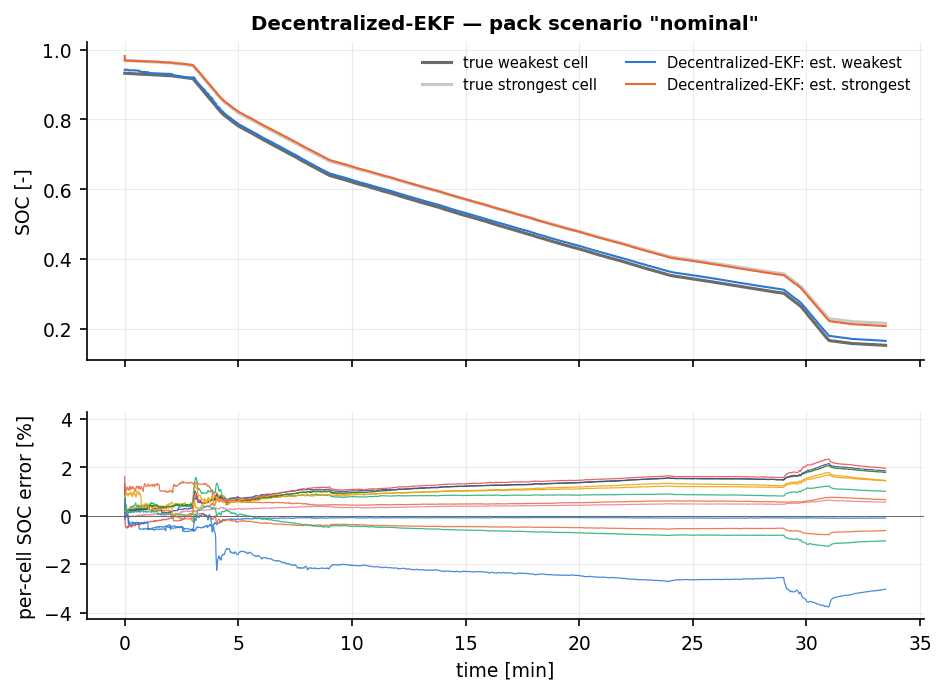
\includegraphics[width=\textwidth]{figures/pack_DecentralizedEKF_nominal.png}
\caption{Decentralized-EKF on the nominal eVTOL mission: twelve independent estimates.}
\end{figure}
\begin{figure}[H]\centering
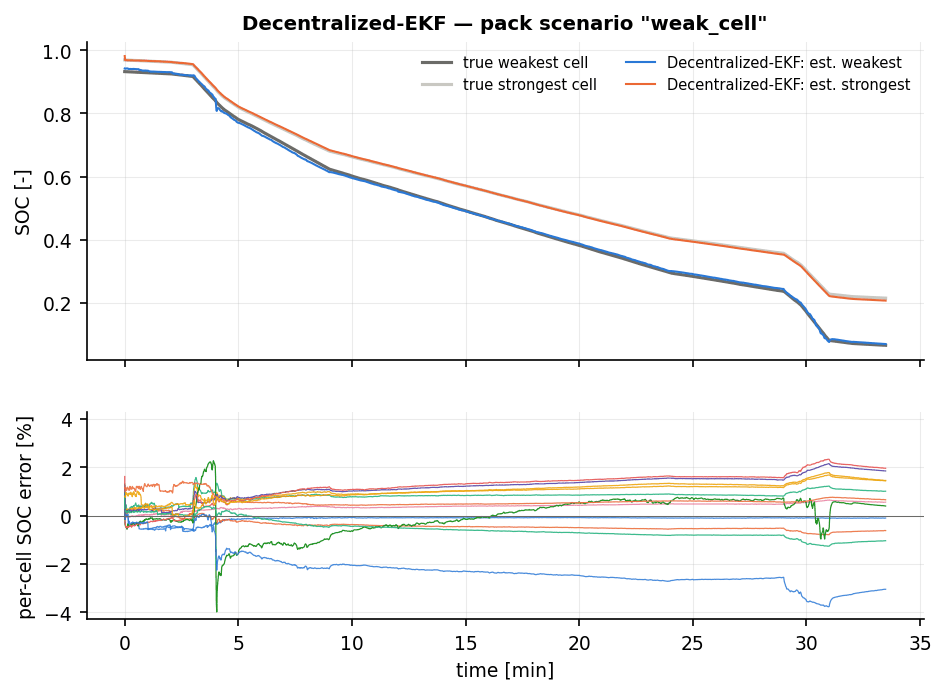
\includegraphics[width=\textwidth]{figures/pack_DecentralizedEKF_weak_cell.png}
\caption{Decentralized-EKF on \texttt{weak\_cell}: cell 5 is tracked by its own filter, which
knows nothing about the other eleven.}
\end{figure}

Means over three seeds of the eVTOL mission:
\begin{center}\small
\begin{tabular}{@{}lcccccc@{}}
\toprule
Scenario & rmse$_{\text{cells}}$ & rmse$_{\min}$ & rmse$_{\text{mean}}$ & ss & max \\
\midrule
\texttt{nominal}          & 0.0123 & 0.0081 & 0.0042 & 0.0134 & 0.046 \\
\texttt{init\_error}      & 0.0118 & 0.0082 & 0.0045 & 0.0129 & 0.042 \\
\texttt{current\_bias}    & 0.0137 & 0.0088 & 0.0072 & 0.0148 & 0.056 \\
\texttt{weak\_cell}       & 0.0129 & 0.0129 & 0.0047 & 0.0137 & 0.048 \\
\texttt{noise\_step}      & 0.0122 & 0.0084 & 0.0041 & 0.0131 & 0.045 \\
\texttt{large\_imbalance} & 0.0174 & 0.0245 & 0.0066 & 0.0179 & 0.061 \\
\bottomrule
\end{tabular}
\end{center}

\paragraph{Reading the baseline.} The steady-state per-cell error settles at
$\approx\num{0.013}$ in every scenario except \texttt{large\_imbalance}, and this figure is
essentially the single-cell EKF floor on this plant: it is set by the model mismatch between the
nominal parameters and each cell's own, which no amount of filtering on one channel removes.
Note the contrast between \texttt{rmse\_cells} (\num{0.0123}) and \texttt{rmse\_mean}
(\num{0.0042}) on \texttt{nominal}: the \emph{average} of the twelve estimates is three times
better than any single one, because the independent voltage-noise components cancel. That
observation is the entire content of Chapters~\ref{ch:bardelta}--\ref{ch:consensus}, which simply
perform the averaging \emph{inside} the filter instead of after it, and consequently reach
$\text{rmse}_{\text{cells}}\approx\num{0.0055}$--\num{0.0066}.

\paragraph{\texttt{init\_error} converges in one sample.} With $\mP_0(\soc,\soc)=\num{0.01}$ and
$R\approx\SI{8.4e-6}{\volt\squared}$, the first measurement update has an SOC gain of
$\approx\num{1.4}$ per volt of innovation, so a \SI{35}{\percent} initial error is removed at
$k=0$; the \texttt{init\_error} row is within \SI{5}{\percent} of \texttt{nominal} for that
reason, and the same holds for every other estimator in this family. The
benchmark's initial-condition test is therefore an \emph{observability} test at $k=0$ rather than
a convergence-rate test; the informative transient scenario here is \texttt{large\_imbalance}.

\paragraph{\texttt{weak\_cell}.} Cell 5 has \SI{12}{\percent} less capacity and \SI{30}{\percent}
more resistance than the nominal parameter set the filter uses. The decentralised filter tracks
it as well as any other cell (\texttt{rmse}$_{\min}=\num{0.0129}$, no divergence) because a
voltage-corrected EKF is insensitive to a capacity error at this level --- but it does so with the
same \num{0.013} floor, whereas the delta-capacity state of Chapter~\ref{ch:bardelta} identifies
the weak cell explicitly and reaches \num{0.0056}.

\section{Summary}
Use the decentralised architecture when the cells do not share a current (parallel groups), when
$N_c$ is small enough that $N_c$ full filters are affordable, or when absolute fault isolation
between channels is required. Expect a per-cell error equal to the single-cell floor, a cost that
scales linearly in $N_c$, and no ability to exploit the fact that $N_c$ sensors are observing
almost the same state. Every other chapter of this family is an attempt to recover that lost
information, and each of them halves the error at between one seventh and one and a half times
the arithmetic.
